\documentclass[tikz,border=7pt]{standalone}
\usetikzlibrary{angles,quotes,calc}
\begin{document}
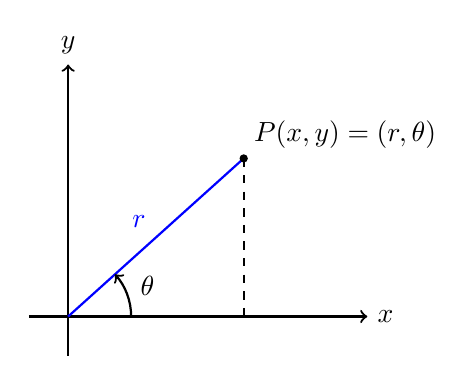
\begin{tikzpicture}[line width=.8pt]
\coordinate (O) at (0,0); \coordinate (X) at (3.5,0); \coordinate (P) at (42:3);
\draw[->] (-.5,0)--(3.8,0) node[right] {$x$}; \draw[->] (0,-.5)--(0,3.2) node[above] {$y$};
\draw[blue,thick] (O)--(P) node[midway,above left] {$r$}; \draw[dashed] (P)--($(O)!(P)!(X)$);
\pic[draw,->,"$\theta$",angle radius=.8cm,angle eccentricity=1.35] {angle=X--O--P};
\fill (P) circle (1.5pt) node[above right] {$P(x,y)=(r,\theta)$};
\end{tikzpicture}
\end{document}
